
\documentclass{beamer}
\usepackage[utf8]{inputenc}

\usetheme{Madrid}
\usecolortheme{default}
\usepackage{amsmath,amssymb,amsfonts,amsthm}
\usepackage{txfonts}
\usepackage{tkz-euclide}
\usepackage{listings}
\usepackage{adjustbox}
\usepackage{array}
\usepackage{tabularx}
\usepackage{gvv}
\usepackage{lmodern}
\usepackage{circuitikz}
\usepackage{tikz}
\usepackage{graphicx}

\setbeamertemplate{page number in head/foot}[totalframenumber]

\usepackage{tcolorbox}
\tcbuselibrary{minted,breakable,xparse,skins}



\definecolor{bg}{gray}{0.95}
\DeclareTCBListing{mintedbox}{O{}m!O{}}{%
  breakable=true,
  listing engine=minted,
  listing only,
  minted language=#2,
  minted style=default,
  minted options={%
    linenos,
    gobble=0,
    breaklines=true,
    breakafter=,,
    fontsize=\small,
    numbersep=8pt,
    #1},
  boxsep=0pt,
  left skip=0pt,
  right skip=0pt,
  left=25pt,
  right=0pt,
  top=3pt,
  bottom=3pt,
  arc=5pt,
  leftrule=0pt,
  rightrule=0pt,
  bottomrule=2pt,
  toprule=2pt,
  colback=bg,
  colframe=orange!70,
  enhanced,
  overlay={%
    \begin{tcbclipinterior}
    \fill[orange!20!white] (frame.south west) rectangle ([xshift=20pt]frame.north west);
    \end{tcbclipinterior}},
  #3,
}
\lstset{
    language=C,
    basicstyle=\ttfamily\small,
    keywordstyle=\color{blue},
    stringstyle=\color{orange},
    commentstyle=\color{green!60!black},
    numbers=left,
    numberstyle=\tiny\color{gray},
    breaklines=true,
    showstringspaces=false,
}
\begin{document}

\title 
{4.3.56}
\date{September 12,2025}


\author 
{EE25BTECH11065-Yoshita J}






\frame{\titlepage}
\begin{frame}{Question}
Find the equation of the plane with intercepts 2, 3 and 4 on the x, y and z - axis respectively.\\

\end{frame}


\begin{frame}{Theoretical Solution}
The intercepts define three points on the plane, which we can label A, B, and C.
\begin{table}[H]    
  \centering
  \begin{table}[h!]
    \centering
    \begin{tabular}{|c|c|}
        \hline
        Point & Coordinates \\
        \hline
	    $A$ & $\myvec{1\\-1}$ \\
	    $B$ & $\myvec{-4\\2k}$ \\
	    $C$ & $\myvec{-k\\-5}$ \\
        \hline
    \end{tabular}
    \caption{Vertices of $\triangle ABC$ before substituting $k$}
    \label{tab:triangle_k}
\end{table}

  \caption{Answers}
  \label{Answers}
\end{table}
\end{frame}

\begin{frame}{Theoretical Solution}
We can find two direction vectors, $\mathbf{m_1}$ and $\mathbf{m_2}$, that lie in the plane:
\begin{align*}
    \mathbf{m_1} &= \mathbf{B} - \mathbf{A} = \myvec{0-2\\3-0\\0-0} = \myvec{-2\\3\\0} \\
    \mathbf{m_2} &= \mathbf{C} - \mathbf{A} = \myvec{0-2\\0-0\\4-0} = \myvec{-2\\0\\4}
\end{align*}
\end{frame}

\begin{frame}{Theoretical Solution}
The normal vector to the plane, $\mathbf{n}$, is found by the cross product of these two vectors.
\begin{align*}
    \mathbf{n} = \mathbf{m_1} \times \mathbf{m_2} &= \myvec{-2\\3\\0} \times \myvec{-2\\0\\4} \\
    &= \myvec{(3)(4) - (0)(0) \\ (0)(-2) - (-2)(4) \\ (-2)(0) - (3)(-2)} = \myvec{12\\8\\6}
\end{align*}
We can simplify the normal vector to $\mathbf{n} = \myvec{6\\4\\3}$. The equation of the plane is then given by:
\[ \mathbf{n}^T (\mathbf{x} - \mathbf{A}) = 0 \]
\end{frame}

\begin{frame}{Theoretical Solution}
Substituting the numerical values, where $\mathbf{x} = [x, y, z]^T$:
\begin{align*}
    \myvec{6 & 4 & 3} \left( \myvec{x\\y\\z} - \myvec{2\\0\\0} \right) &= 0 \\
    \implies \myvec{6 & 4 & 3} \myvec{x-2\\y\\z} &= 0 \\
    \implies 6(x-2) + 4y + 3z &= 0 \\
    \implies 6x - 12 + 4y + 3z &= 0 \\
    \implies 6x + 4y + 3z &= 12
\end{align*}
\end{frame}


\begin{frame}[fragile]
    \frametitle{C Code}

    \begin{lstlisting}
#include <stdio.h>

typedef struct {
    double x, y, z;
} Vector;

typedef struct {
    double a, b, c, d;
} Plane;

Vector subtract_vectors(Vector v1, Vector v2) {
    Vector result;
    result.x = v1.x - v2.x;
    result.y = v1.y - v2.y;
    result.z = v1.z - v2.z;
    return result;
}


    \end{lstlisting}
\end{frame}

\begin{frame}[fragile]
    \frametitle{C Code}

    \begin{lstlisting}
Vector cross_product(Vector v1, Vector v2) {
    Vector result;
    result.x = v1.y * v2.z - v1.z * v2.y;
    result.y = v1.z * v2.x - v1.x * v2.z;
    result.z = v1.x * v2.y - v1.y * v2.x;
    return result;
}

double dot_product(Vector v1, Vector v2) {
    return v1.x * v2.x + v1.y * v2.y + v1.z * v2.z;
}

    \end{lstlisting}
\end{frame}
\begin{frame}[fragile]
    \frametitle{C Code}

    \begin{lstlisting}
Plane find_plane_equation(Vector p1, Vector p2, Vector p3) {
    Vector m1 = subtract_vectors(p2, p1);
    Vector m2 = subtract_vectors(p3, p1);
    Vector normal = cross_product(m1, m2);
    double d = dot_product(normal, p1);

    Plane result;
    result.a = normal.x;
    result.b = normal.y;
    result.c = normal.z;
    result.d = d;
    return result;
}


    \end{lstlisting}
\end{frame}

\begin{frame}[fragile]
    \frametitle{Python Code}
    \begin{lstlisting}
import numpy as np
import matplotlib.pyplot as plt

def get_z(x, y):
    return (12 - 6*x - 4*y) / 3

x_vals = np.linspace(0, 4, 10)
y_vals = np.linspace(0, 5, 10)
x_grid, y_grid = np.meshgrid(x_vals, y_vals)
z_grid = get_z(x_grid, y_grid)

fig = plt.figure(figsize=(8, 6))
ax = fig.add_subplot(111, projection='3d')

ax.plot_surface(x_grid, y_grid, z_grid, alpha=0.7, cmap='viridis')
    \end{lstlisting}
\end{frame}

\begin{frame}[fragile]
    \frametitle{Python Code}
    \begin{lstlisting}
  ax.scatter(2, 0, 0, color='red', s=100, label='Intercept (2,0,0)')
ax.scatter(0, 3, 0, color='green', s=100, label='Intercept (0,3,0)')
ax.scatter(0, 0, 4, color='blue', s=100, label='Intercept (0,0,4)')

ax.set_xlabel('X-axis')
ax.set_ylabel('Y-axis')
ax.set_zlabel('Z-axis')
ax.set_title('Plane: 6x + 4y + 3z = 12')
ax.legend()
plt.grid(True)
plt.show()
  
   
    \end{lstlisting}
\end{frame}


\begin{frame}{Plot}
    \centering
    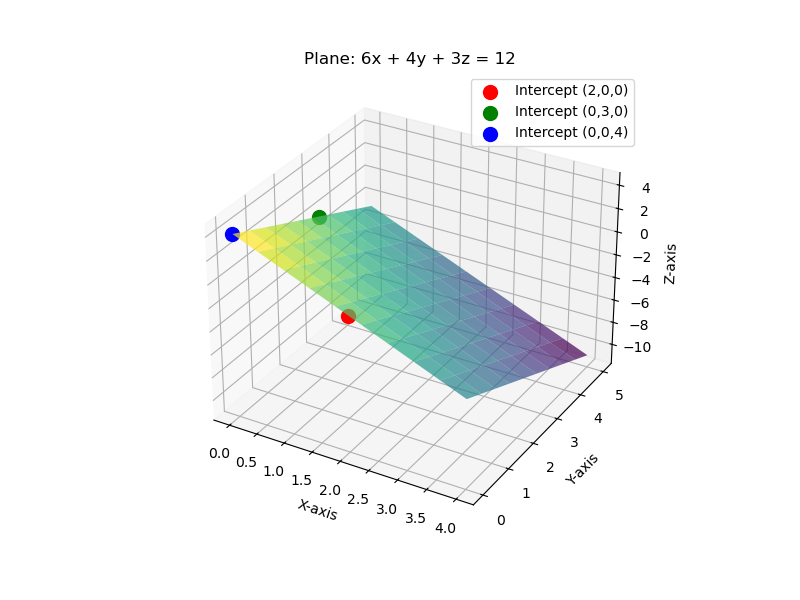
\includegraphics[width=\columnwidth, height=0.8\textheight, keepaspectratio]{figs/fig2.png}     
\end{frame}


\end{document}
